\documentclass[../thesis]{subfiles}

\begin{document}
	\section{Architecture}
	\label{sec:cuda:arch}

	\begin{figure}[!htp]
		\centering
		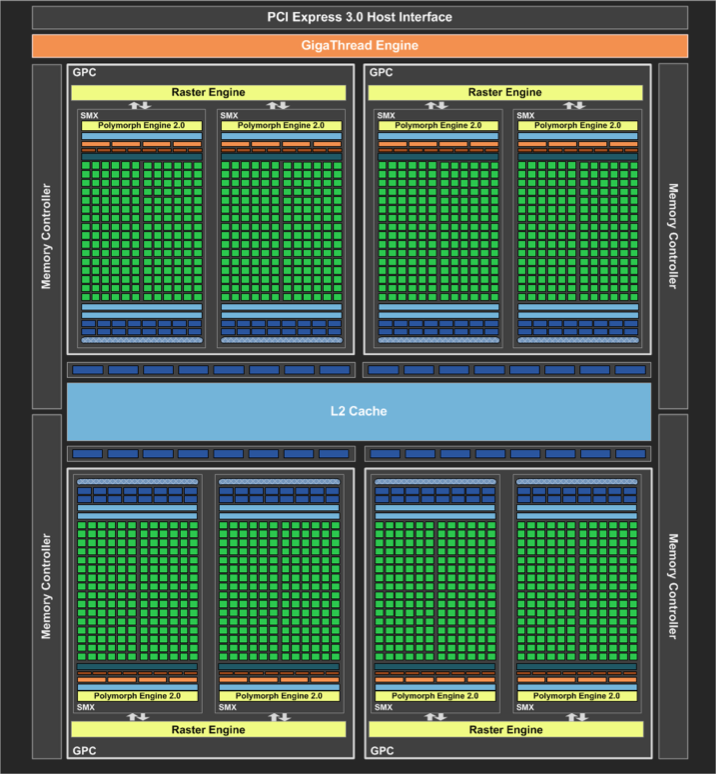
\includegraphics[width=0.8\textwidth]{assets/images/cuda/arch/gtx680.png}
		\caption[Overview of the GeForce GTX 680 Kepler Architecture]{Overview of the GeForce GTX 680 Kepler Architecture \cite{NVIDIA:GTX680}}
		\label{fig:gtx680}
	\end{figure}
	
	\begin{wrapfigure}{r}{0.3\textwidth}
		\centering
		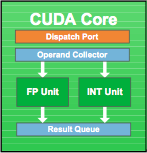
\includegraphics[width=0.25\textwidth]{assets/images/cuda/arch/cuda-core.png}
		\caption{CUDA core diagram}
		\label{fig:cudacore}
	\end{wrapfigure}

	\cuda-enabled \gpus are composed by several building blocks called \gpcs, each with multiple multithreaded \sms connected to the global device memory (GDDR5 DRAM). Each \sm contains
	\begin{itemize}
		\item a large set of \cuda cores, the processing units that perform the arithmetic operations;
		\item a much more limited number of \sfus and Load/Store units;
		\item a Register File, big enough to provide each thread with a many registers (255 in recent generations \cite{NVIDIA:KEPLER});
		\item Level 1 data cache, shared among all cores;
		\item shared memory;
		\item schedulers to map threads to the cores for execution;
		\item instruction cache shared among the schedulers;
	\end{itemize}

	In \cuda, a kernel represents a set of instructions to be executed as a parallel task. These parallel tasks are constituted by a set of \cuda threads, which execute the same instructions on different data (follow both \simd and \simt approaches). \cuda threads are organized in a hierarchy: blocks aggregate threads assigned to the same \sm, and the set of all the blocks running the same kernel is a grid.

	\begin{wrapfigure}{r}{0.4\textwidth}
		\centering
		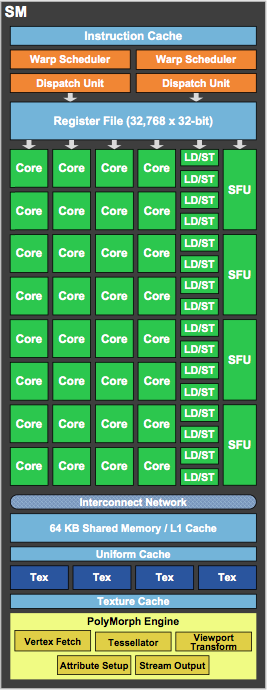
\includegraphics[width=0.3\textwidth]{assets/images/cuda/arch/sm.png}
		\captionsetup{font=small}
		\caption{Streaming Multiprocessor diagram for the GF100 architecture}
		\label{fig:gf100}
	\end{wrapfigure}

	Inside a \sm, the scheduler groups up to 32 threads from the same block into warps, which are then set to run on the \sm at a given time. Since warps group threads running the same instruction of the kernel at any given time, conditional jumps are very expensive. When a conditional jump is met, if divergence occurs, it causes the two conditional branches to be executed consecutively, doubling the warp execution time.

	While scheduling warps for execution, the scheduler holds them in a scoreboard waiting for data and issues warps containing those ready for execution with very low switching time. For this reason, these devices benefit from having a lot more threads than those able to run concurrently, as it helps hiding the memory latency.

	When accessing memory in a \cuda kernel, coalesced memory accesses are required in order to achieve an efficient memory usage. Coalesced accesses happen when the threads in a warp access global memory at the same time asking for contiguous addresses. Since the load units are able to retrieve data from memory in blocks, this results in more data being fetched with less accesses. Coalesced accesses also help the memory controller to find the best grouping of threads to merge the requests into fewer memory accesses.

	\gpus implementing the G80 architecture, the first \cuda-enabled devices, had a memory bandwidth of 86.4 GB/s. On the other hand, modern \gpus using \pcie Generation 3 interface can transfer data between global memory and the system main memory at 8 GB/s in each direction (at the same time) \cite{PMPP:2012}. Since communication with the \cpu is so expensive it must be kept to a minimum in order to maximize performance.

	\subfile{tex/621.cuda.arch.kepler.tex}
\end{document}
